\chapter[L'application]{Présentation de l'application}

Dans ce chapitre on présente l'application Crazy wolf. 
Au traver d'images commentées nous allons décrire plusieurs scénarios
d'utilisation.
\section[Authentification \& écran d'accueil - Scénario I]{Scénario I}
\subsection*{Authentification \& écran d'accueil}
Ici la serveuse Kim, qui n'a pas de privilèges, c'est-à-dire qu'elle n'est 
ni manager ni administratice, se connecte et accède au premier écran possible.
Puis elle, click sur "Mes services".

\begin{figure}[!h]
    \centering
    \begin{subfigure}{.3\textwidth}
        \centering
        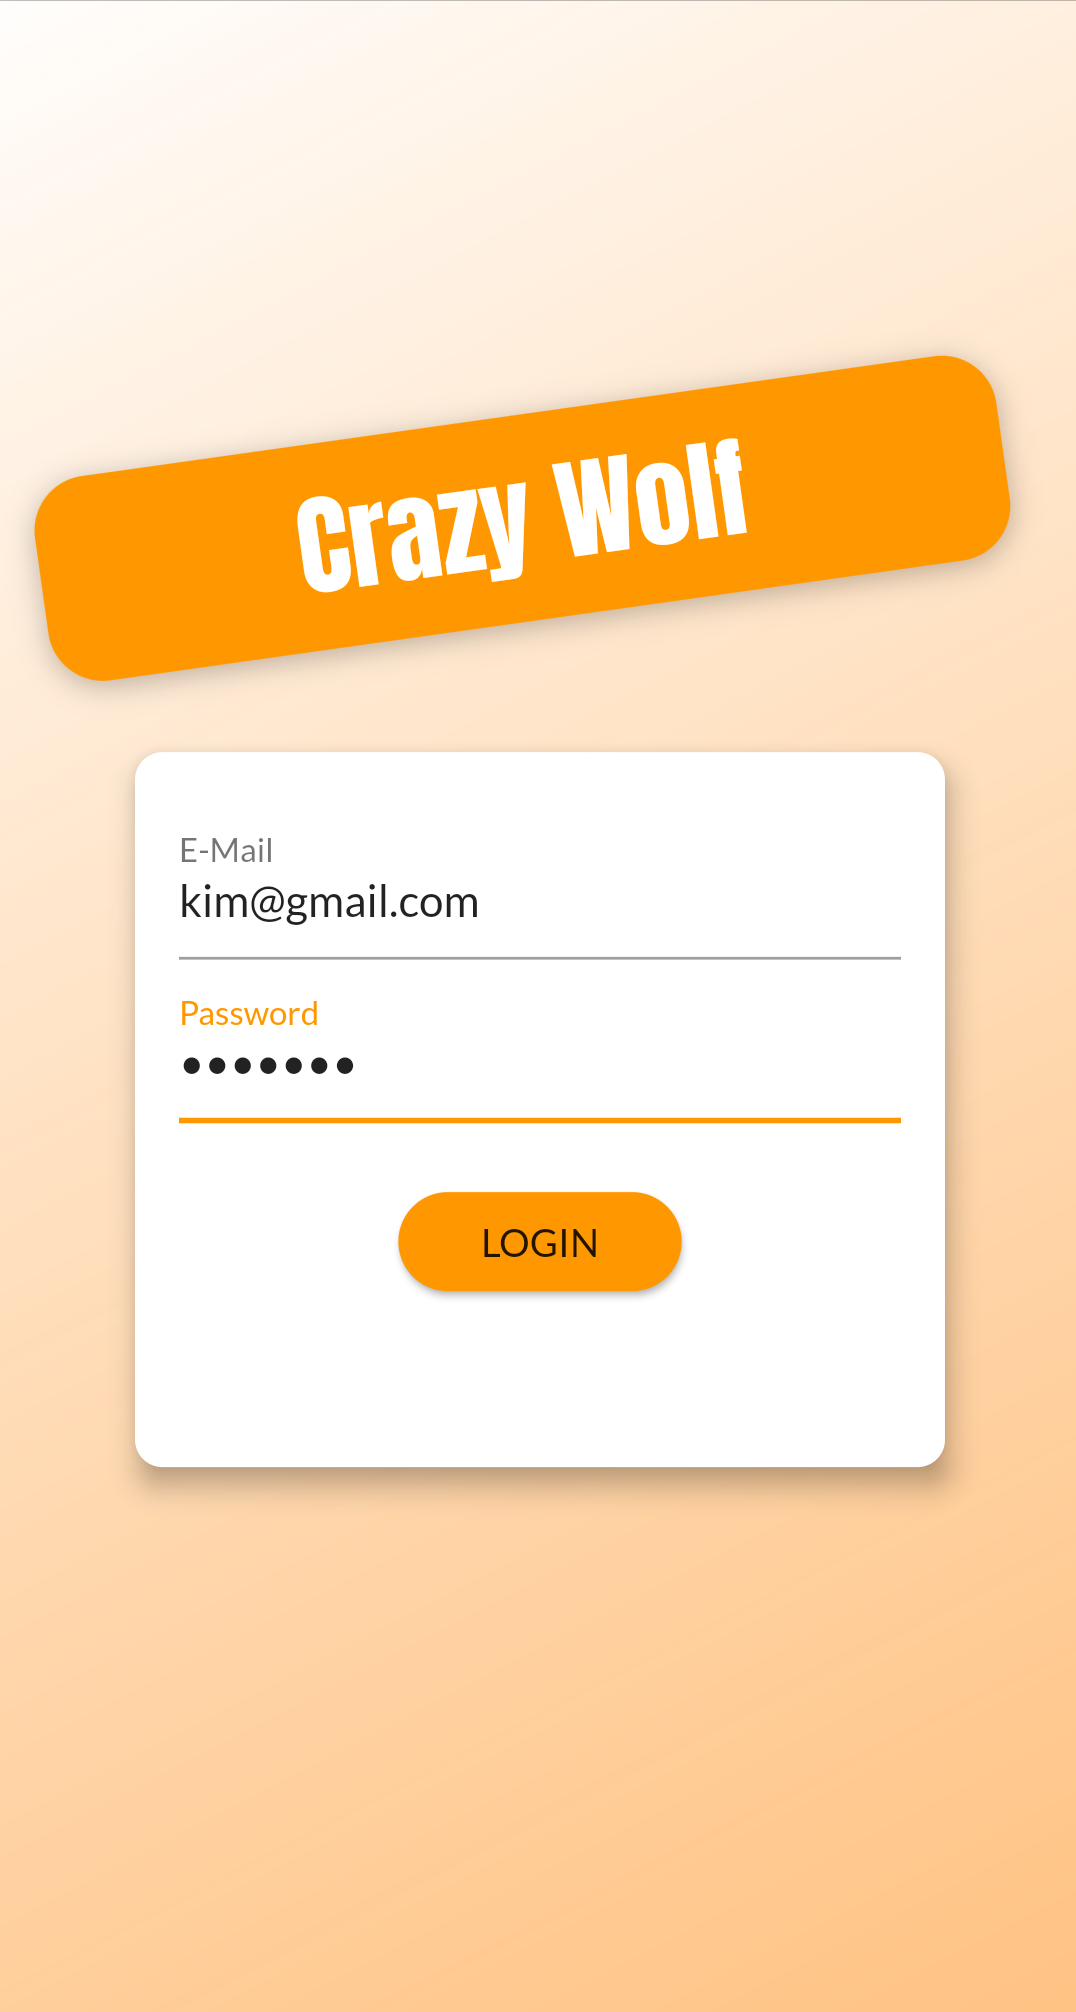
\includegraphics[width=0.9\linewidth]{screenshots/scenario_01/login.png}
        \caption{login}
        \label{fig:login}
    \end{subfigure}
    \begin{subfigure}{.3\textwidth}
        \centering
        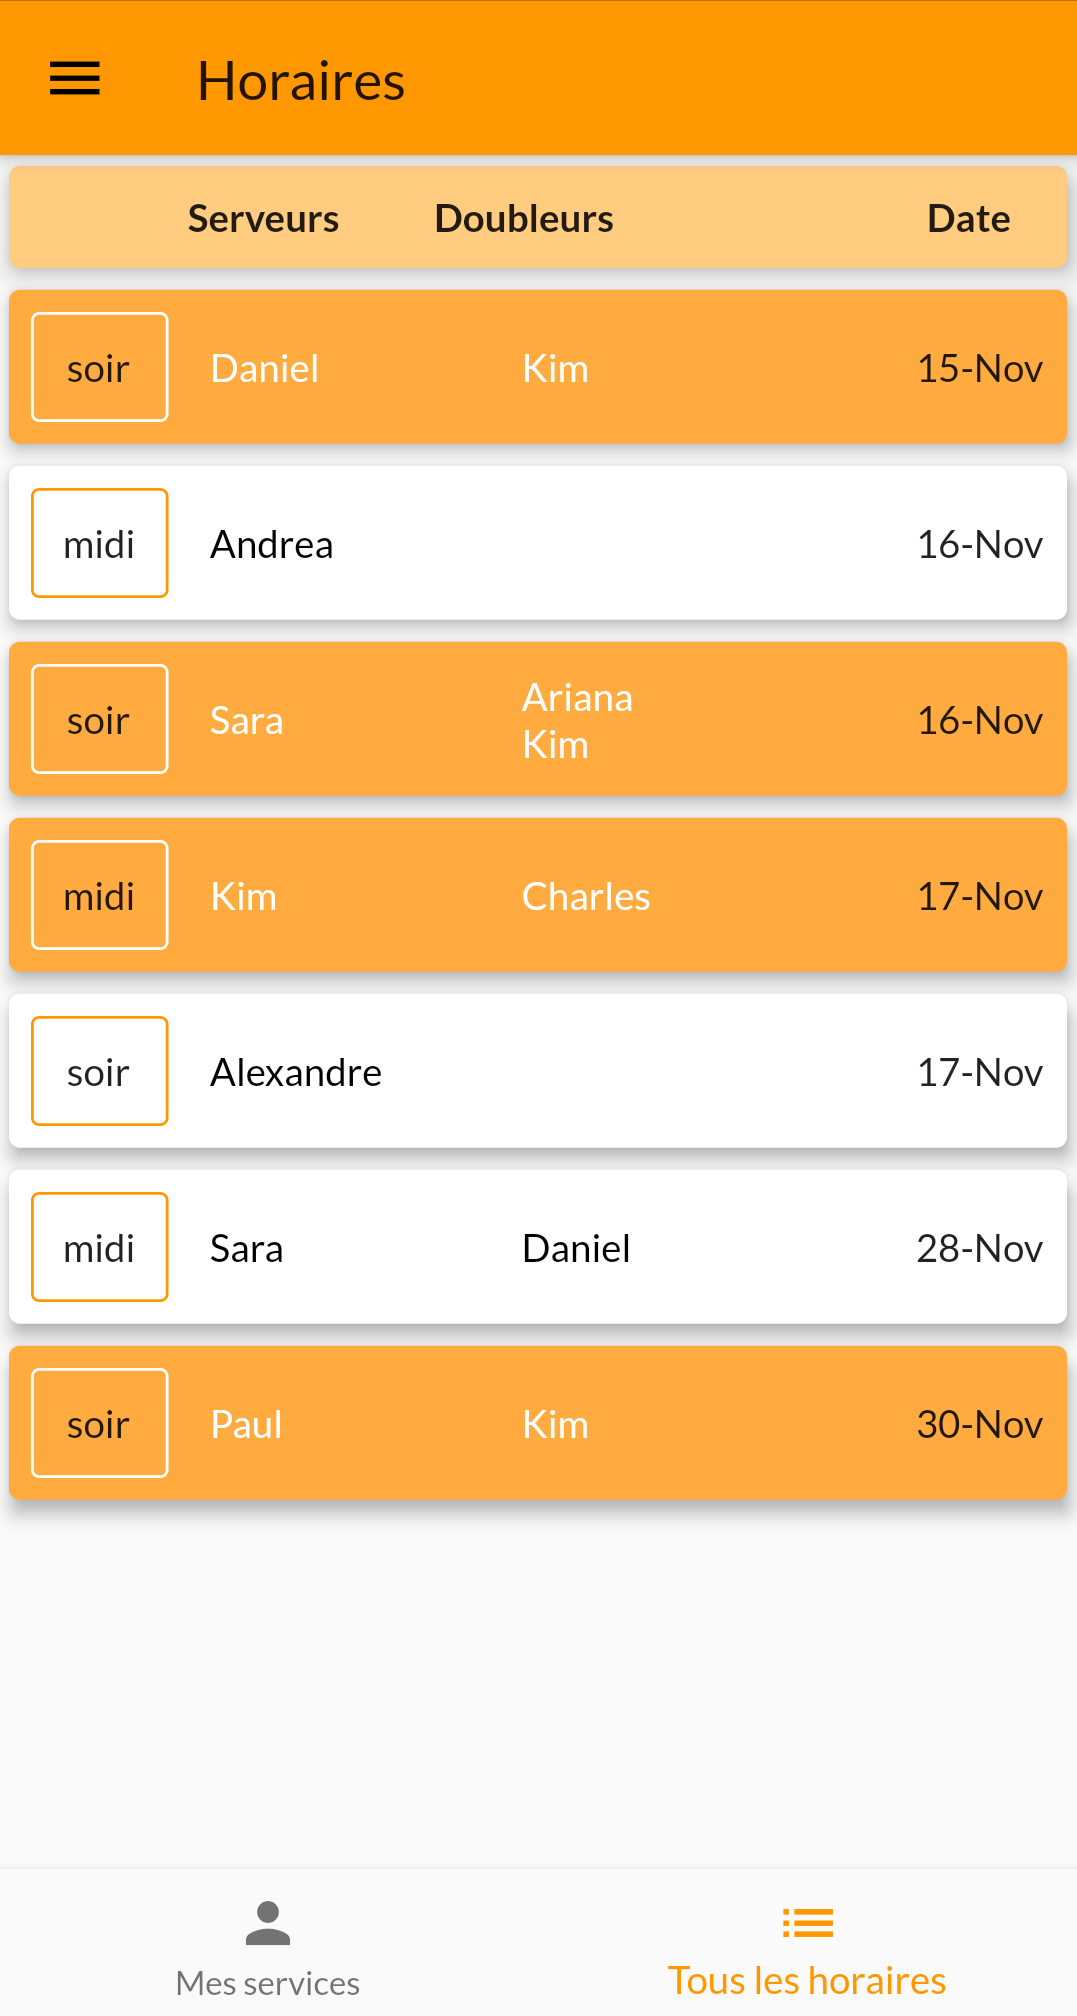
\includegraphics[width=0.9\linewidth]{screenshots/scenario_01/horaires.png}
        \caption{horaires}
        \label{fig:horaires}
    \end{subfigure}
    \begin{subfigure}{.3\textwidth}
        \centering
        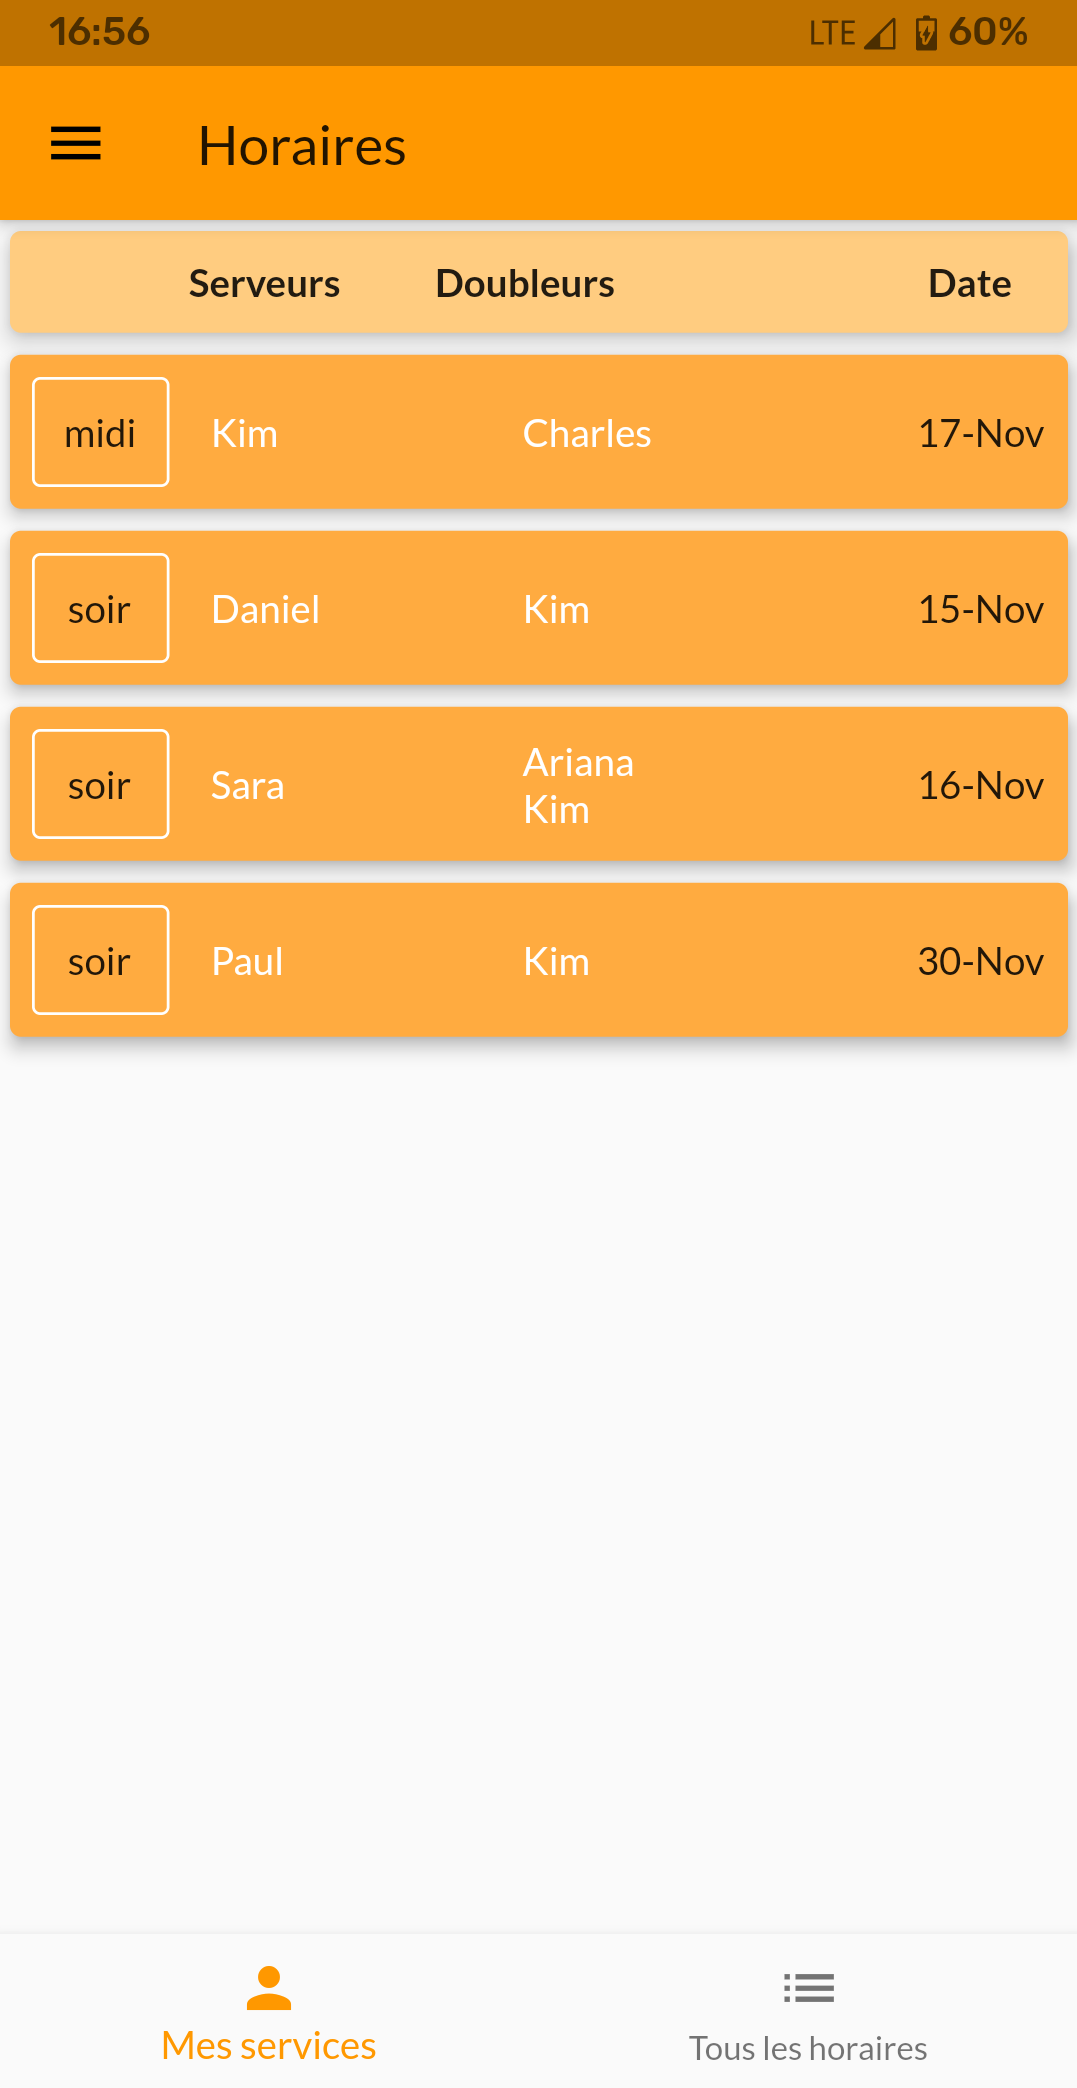
\includegraphics[width=0.9\linewidth]{screenshots/scenario_01/mesHoraires.png}
        \caption{mes horaires}
        \label{fig:mesHoraires}
    \end{subfigure}
    \caption{scénario I}
    \label{fig:scen01}
\end{figure}

L'utilisateur doit dans un premier temps se connecter à l'aide d'identifiants déjà existant dans l'écran \ref{fig:login}. Une fois l'addresse mail et le mot de passe saisis, 
l'écran \ref{fig:horaires} s'affiche. 


On y voit l'ensemble des horaires de travail. Les services sont définis par
\begin{itemize}
    \item le type: midi ou soir.
    \item un ou plusieurs serveurs.
    \item zero, un ou plusieurs doubleurs.
    \item la date
\end{itemize}
Les services sont ordonnés par date, les jours précédents au moment de la connection ne 
sont pas affichés. Les horaires correspondant à la personne authentifié sont de couleurs orange.

Les services sont affichés sous forme de liste scrollable.

On peut également naviguer à l'aide du menu inférieur à "mes services" où seuls les horaires du serveur authentifié sont affichés. Comme on le voit 
dans \ref{fig:mesHoraires}

\section[Mise en bourse d'un service - Scénario II]{Scénario II}
    \subsection*{Mise en bourse d'un service}
    Supposons que Kim, la serveuse authentifiée ne puisse pas travailler le 17 novembre.
    Elle souhaite donc se faire remplacer. Pour se faire, dans l'onglet 
    "horaires", elle peut mettre son service en bourse en glissant le 
    service en question sur la gauche.
    \begin{figure}[!h]
        \centering
        \begin{subfigure}{.45\textwidth}
            \centering
            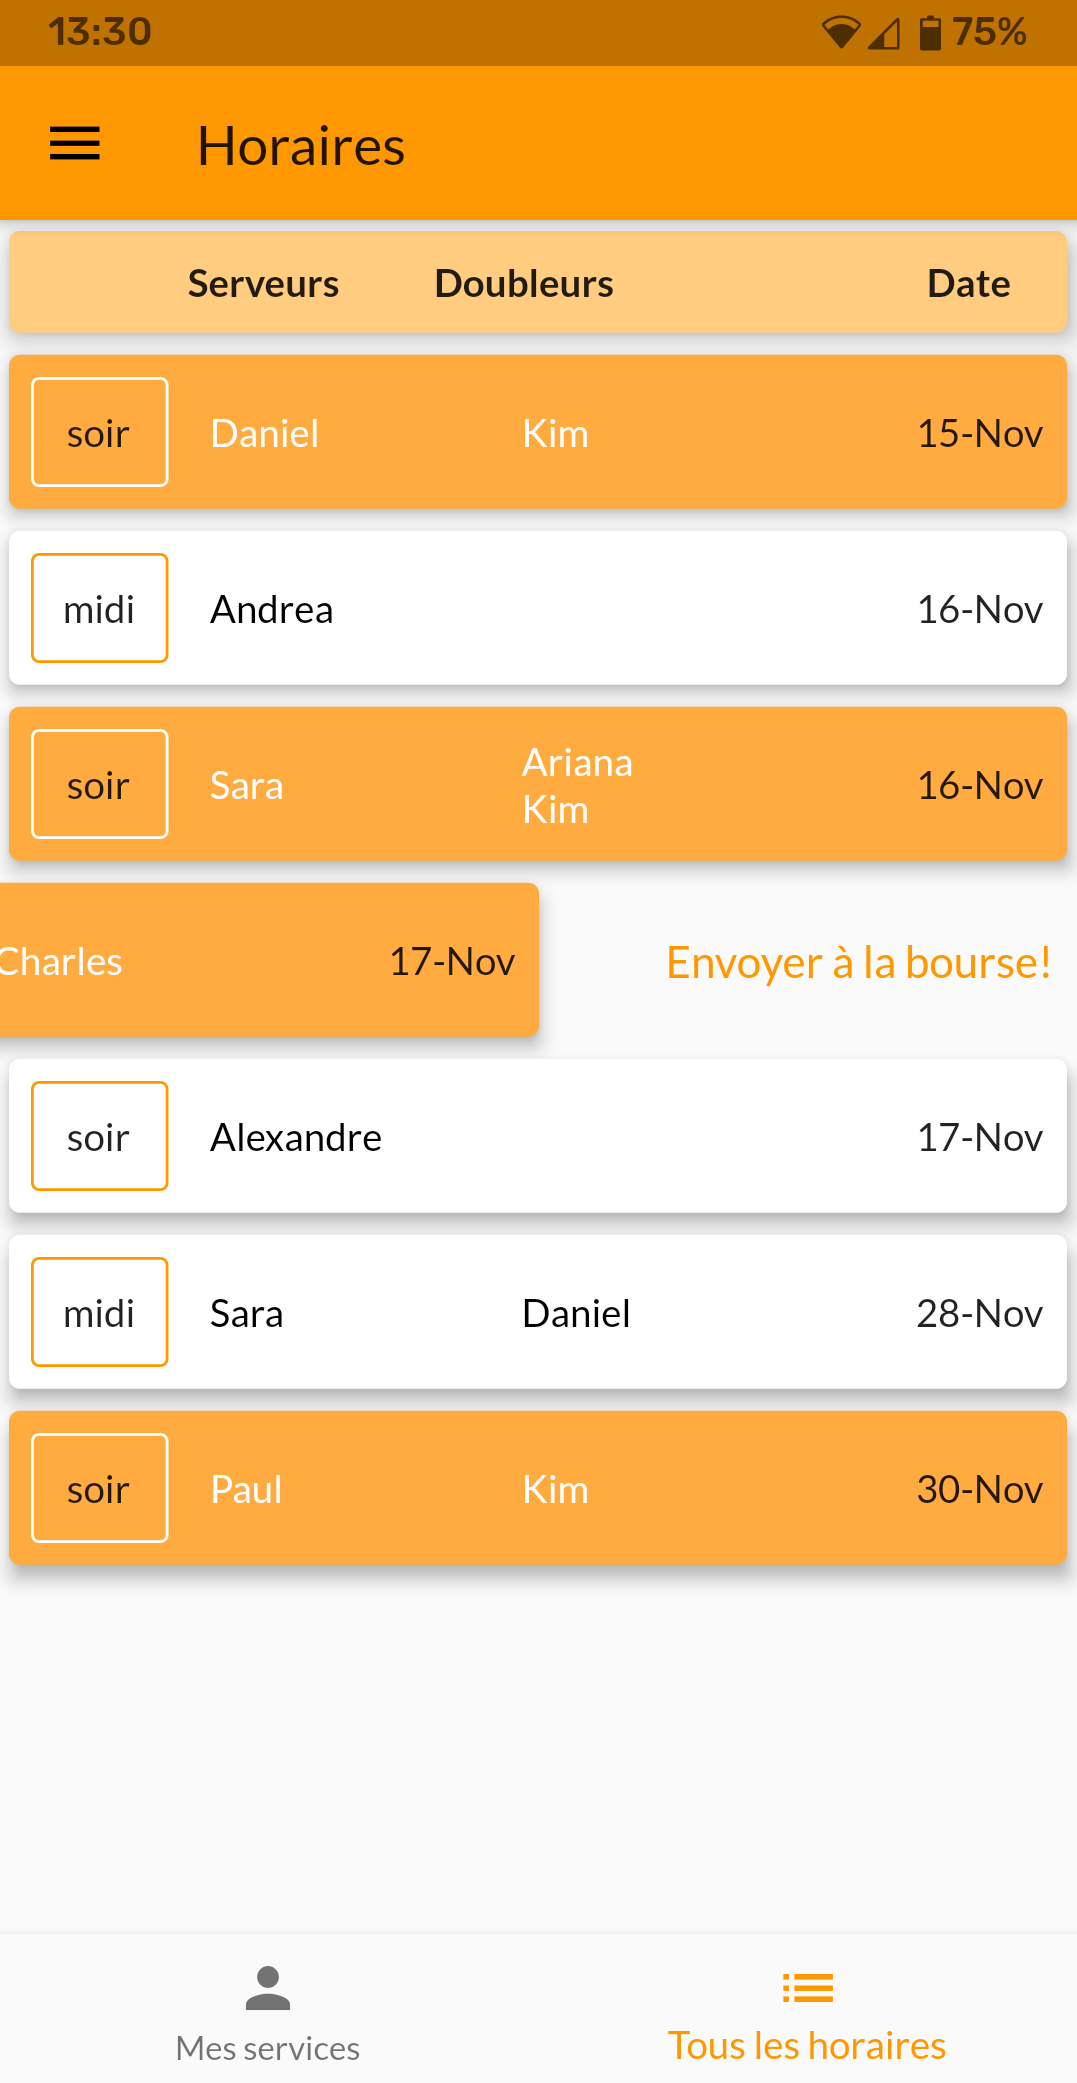
\includegraphics[width=0.6\linewidth]{screenshots/scenario_02/mise_en_bourse.png}
            \caption{mise en bourse}
            \label{fig:mise_en_bourse}
        \end{subfigure}
        \begin{subfigure}{.45\textwidth}
            \centering
            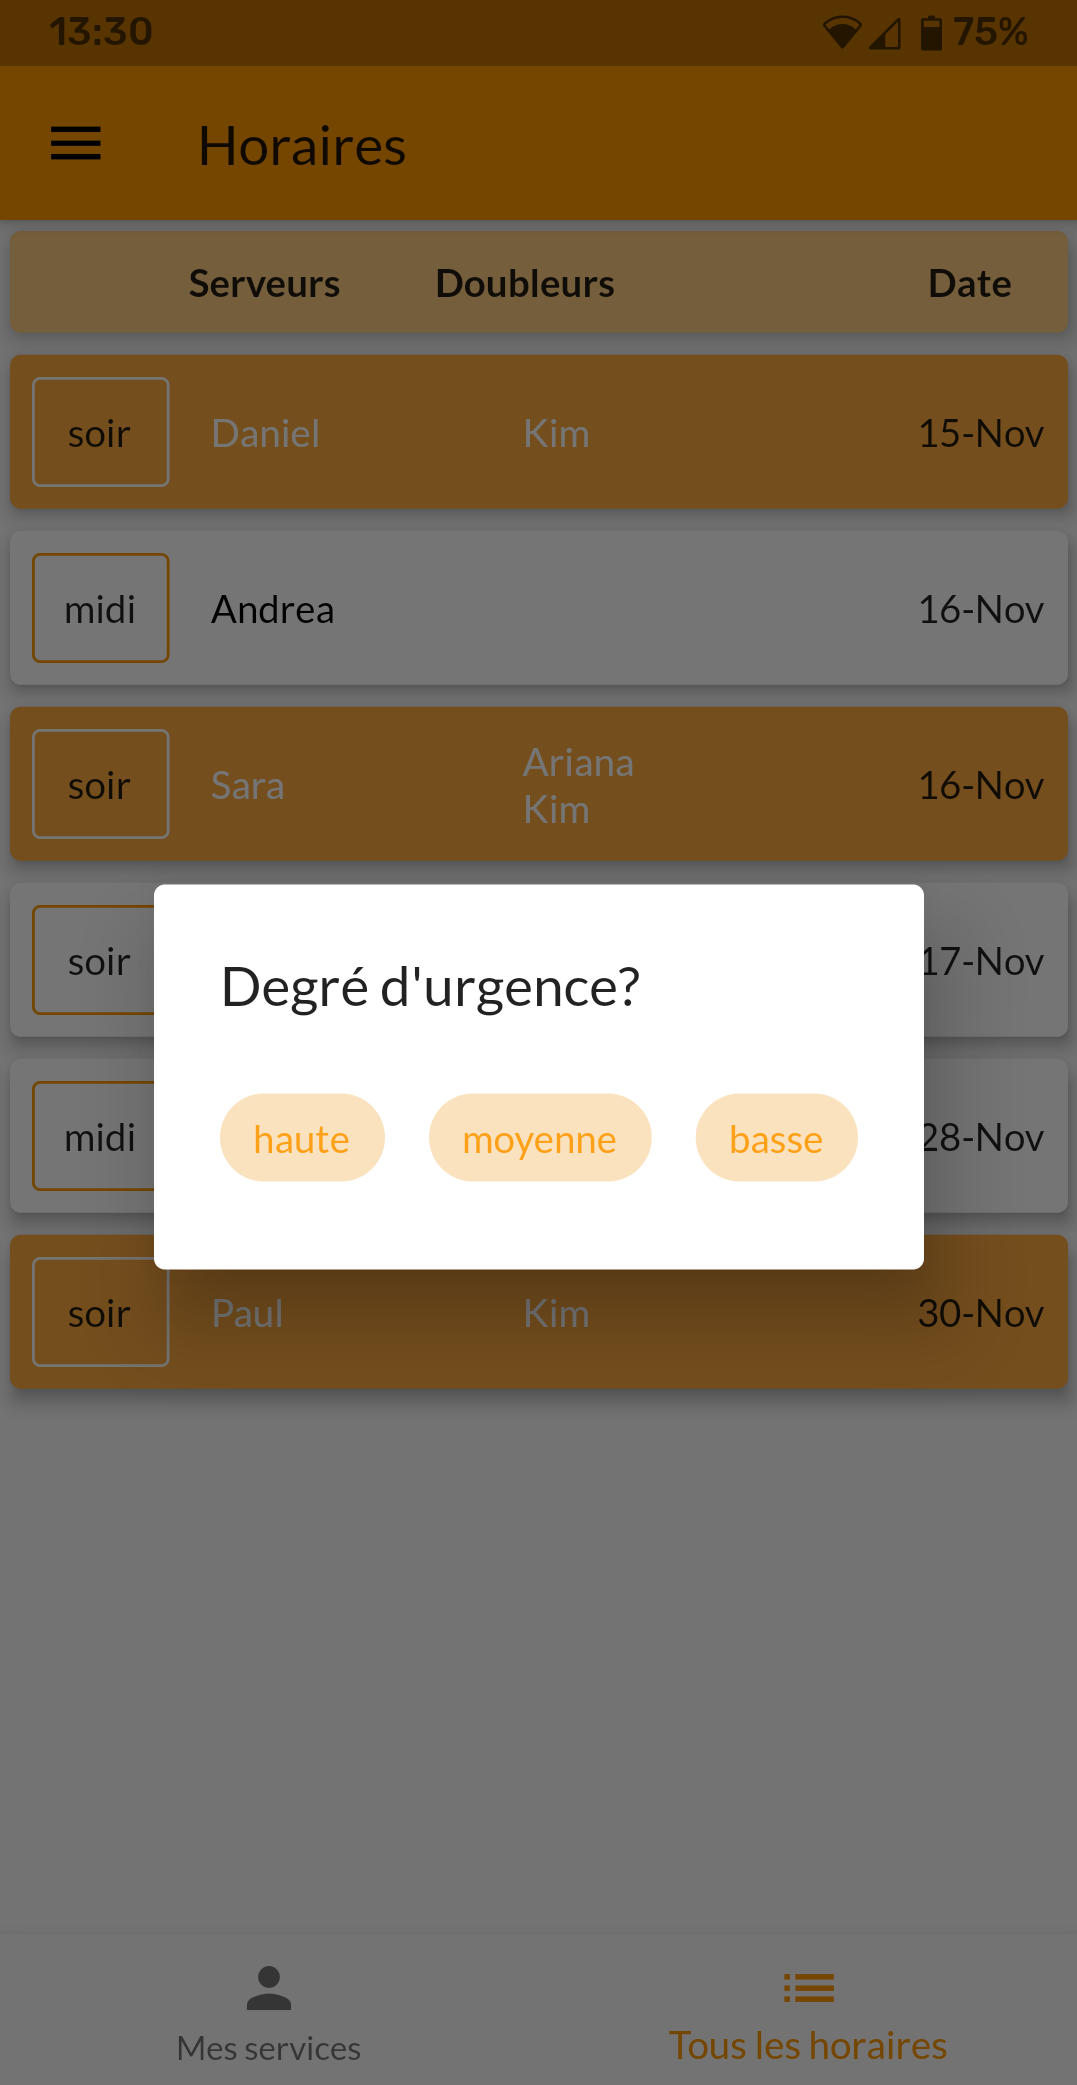
\includegraphics[width=0.6\linewidth]{screenshots/scenario_02/urgence.png}
            \caption{urgence}
            \label{fig:urgence}
        \end{subfigure}
        \caption{scénario II - a}
        \label{fig:scen02a}
    \end{figure}

Une fois le glissement éffectué un popup est s'affiche \ref{fig:urgence} demandant
à quel point le remplacement est urgent. Une fois que l'utilisateur à répondu, le service est mis
en bourse. Un snakbar s'affiche pour le notifier que l'action à réussi.

Si l'action est réussie, tous les utilisateur de l'application sont notifié \ref{fig:notif} comme quoi un 
nouveau service est disponible. La notification informe sur la disponibilité d'un service ainsi que 
l'urgence requise à y répondre. 

Suit à ça, l'utilisatrice peut naviguer à l'aide du menu lateral \ref{fig:menu_sans_droits} où s'affichent les options
de navigation suivante: 
\begin{itemize}
    \item Horaires: Pour aller à l'écran "Horaires" \ref{fig:horaires}
    \item Logout: Pour se déconnecter, qui revoit à l'écran \ref{fig:login}
    \item Bourse: Pour aller à l'écran bourse aux jobs \ref{fig:bourse}
\end{itemize}
\begin{figure}[!h]
    \begin{subfigure}[]{.3\textwidth}
        \centering
        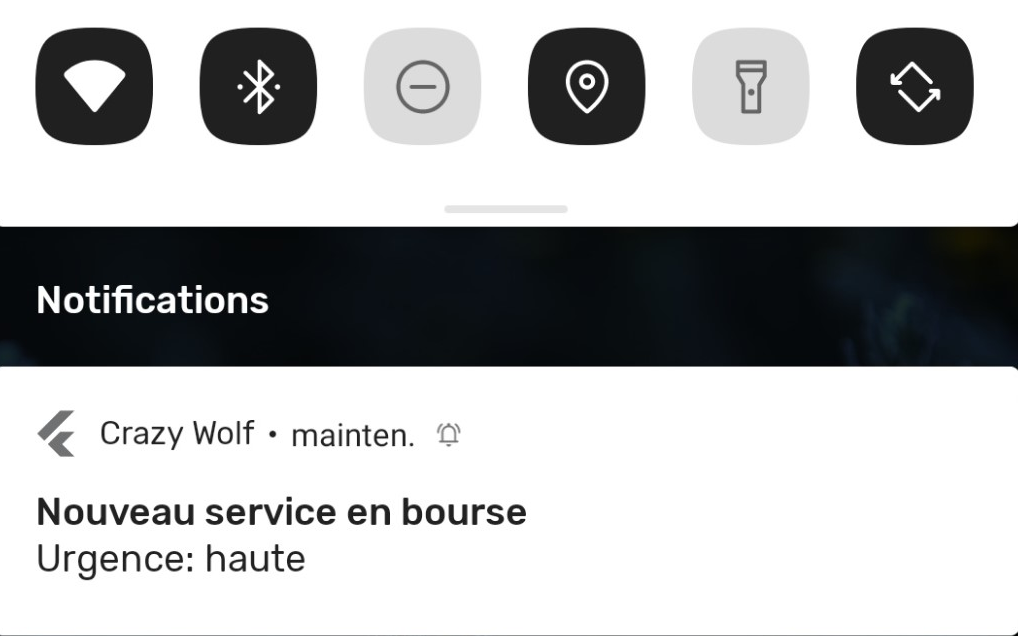
\includegraphics[width=0.9\linewidth]{screenshots/scenario_02/notification.png}
        \caption{notification}
        \label{fig:notif}
    \end{subfigure}
    \centering
    \begin{subfigure}{.3\textwidth}
        \centering
        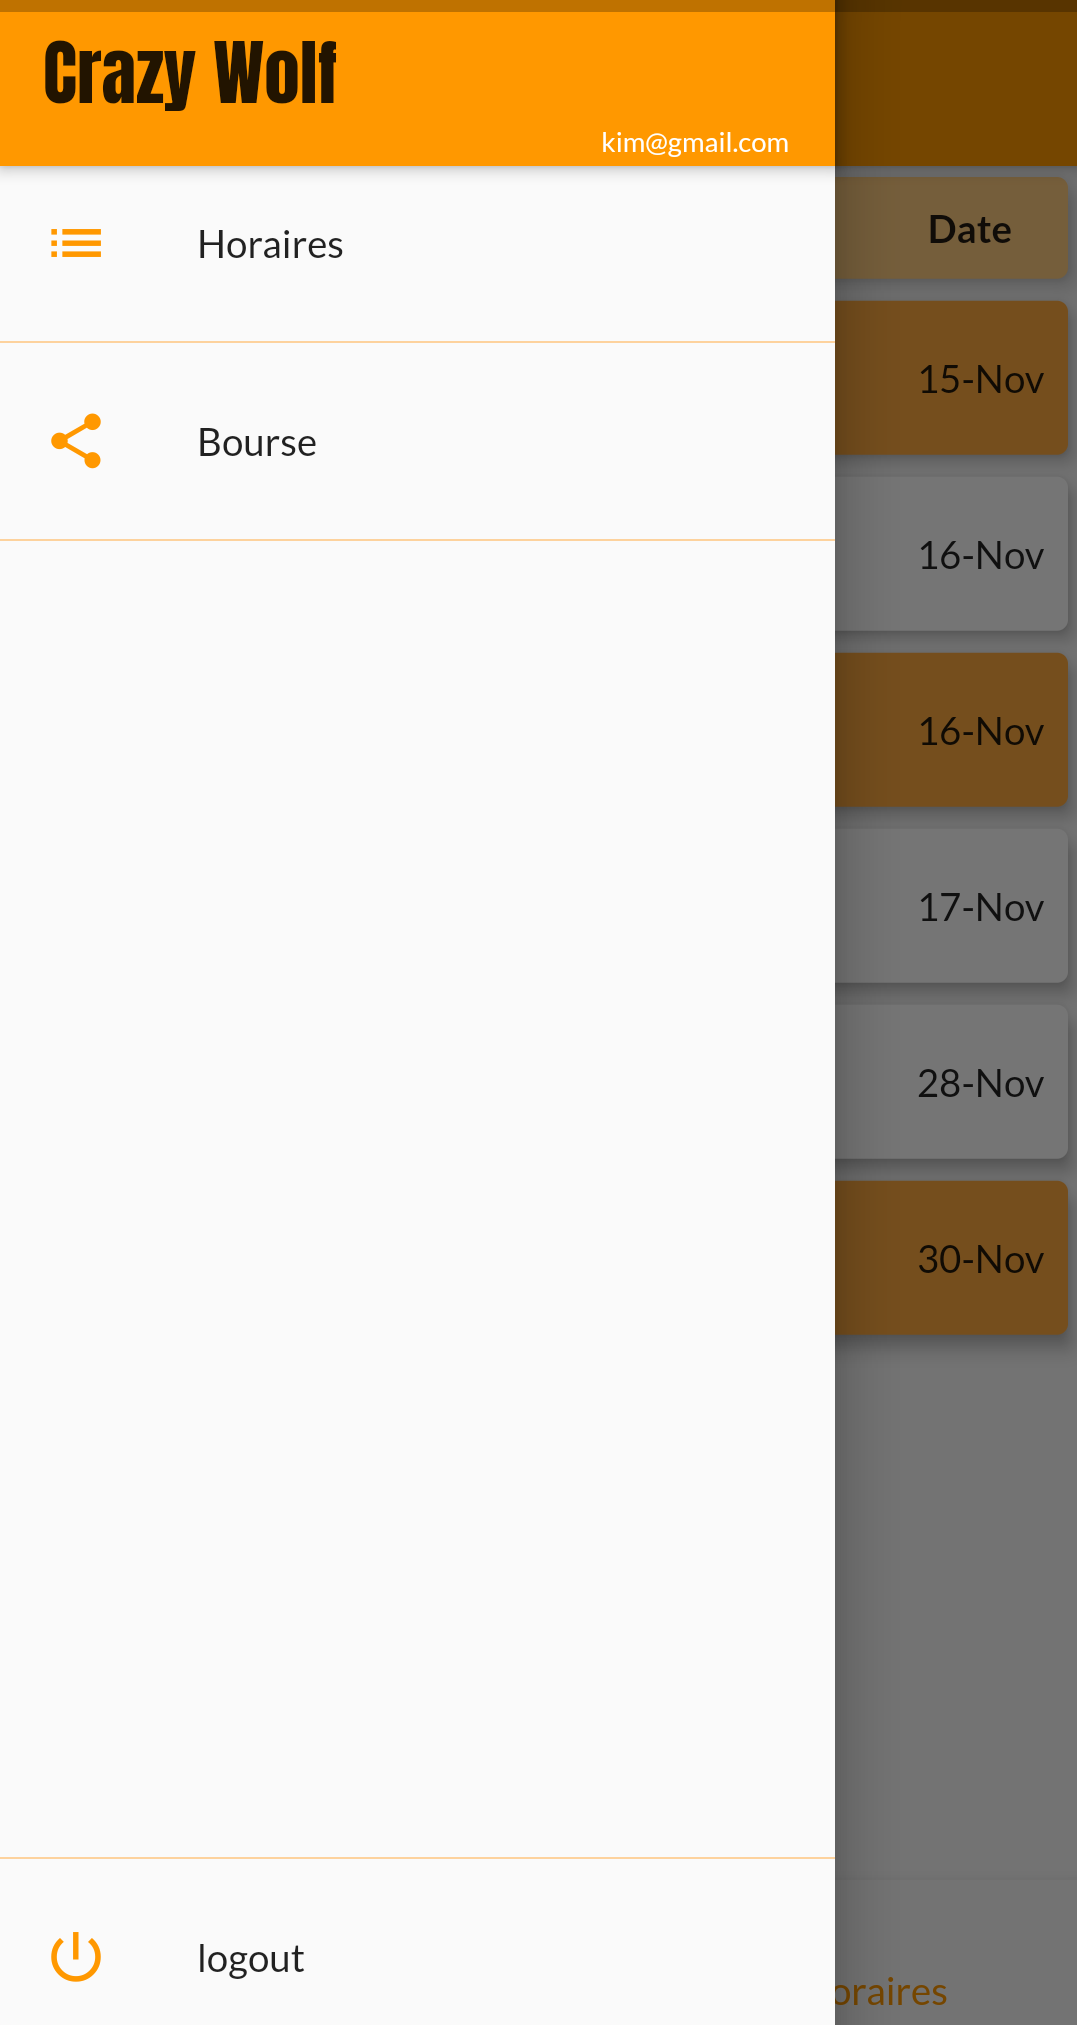
\includegraphics[width=0.9\linewidth]{screenshots/scenario_02/menu_serveur_normal.png}
        \caption{menu sans privilèges}
        \label{fig:menu_sans_droits}
    \end{subfigure}
    \begin{subfigure}{.3\textwidth}
        \centering
        
\includegraphics[width=0.9\linewidth]{screenshots/scenario_02/bourse_jobs.png}
        \caption{bourse}
        \label{fig:bourse}
    \end{subfigure}
    \caption{scénario II - b}
    \label{fig:scen02b}
\end{figure}

Dans l'onglet "Bourse aux jobs" son service est disponible à toute personne souhaitant y postuler. 
Cet onglet est partagé parmis tous les utilisateurs de l'application.

La couleur représente le degré d'urgence. Ainsi la convention suivante est appliqué:
\begin{itemize}
    \item rouge: implique une urgence élevée.
    \item jaune: implique une urgence moyenne.
    \item vert: implique une urgence basse.
\end{itemize}

L'onglet "Bourse aux jobs" affiche tous les service actuellement en bourse sous
forme de liste scrollable. L'utilisateur ayant mis son service en bourse
doit patienter à ce que quelqu'un y postule.

Les utilisateur sans privilèges sont authorisé à mettre un service en bourse uniquement s'ils y travaillent.

\section[Postuler pour un service - Scénario III]{Scénario III}
    \subsection*{Postuler pour un service}
    Dans la continuation du scénario précédent, après avoir été notifiés,
    deux serveurs vont postuler au nouveau service mis
    en bourse. Leurs parcours étant identiques, nous allons en montrer qu'un.
    Supposons qu'ils se soient authentifié comme vu en \ref{fig:login} et qu'ils se trouvent
    dans l'onglet "Bourse au jobs" \ref{fig:bourse}.

    \begin{figure}[h]
        \centering
        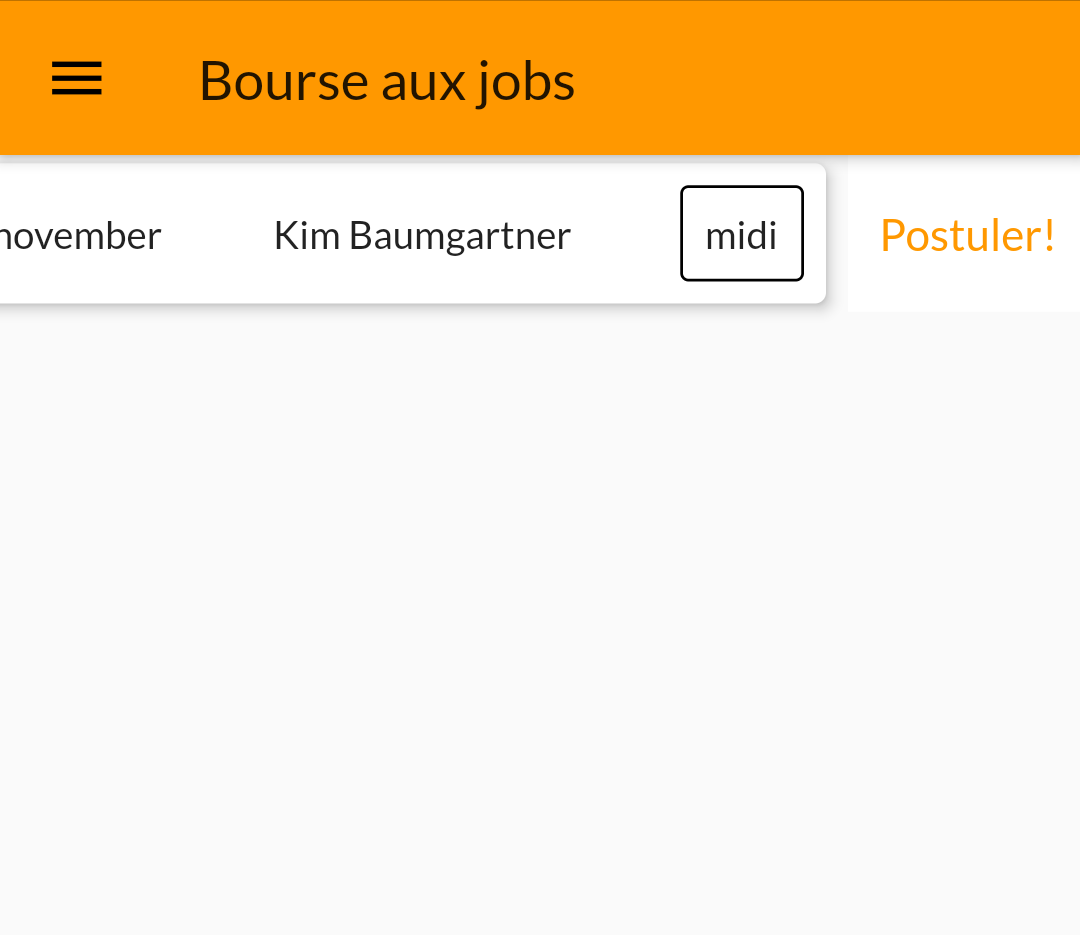
\includegraphics[width=.3\linewidth]{screenshots/scenario_03/postuler.png}
        \caption{postuler}
        \label{fig:postuler}
    \end{figure}

    Alors, ils peuveunt glisser le service auquel ils souhaitent postuler sur
    la gauche. À nouveau, si l'opération réussi, un snackbar apparaît pour l'indiquer.

    L'utilisateur ayant mis le service en bourse doit procéder à l'acceptation
    d'un seul postulant. Dans "Bourse aux jobs" \ref{fig:bourse} les éléments de 
    la liste sont clickable. Lorsqu'un utilisateur click deux options sont possibles:

    \begin{figure}[!h]
        \centering
        \begin{subfigure}{.45\textwidth}
            \centering
            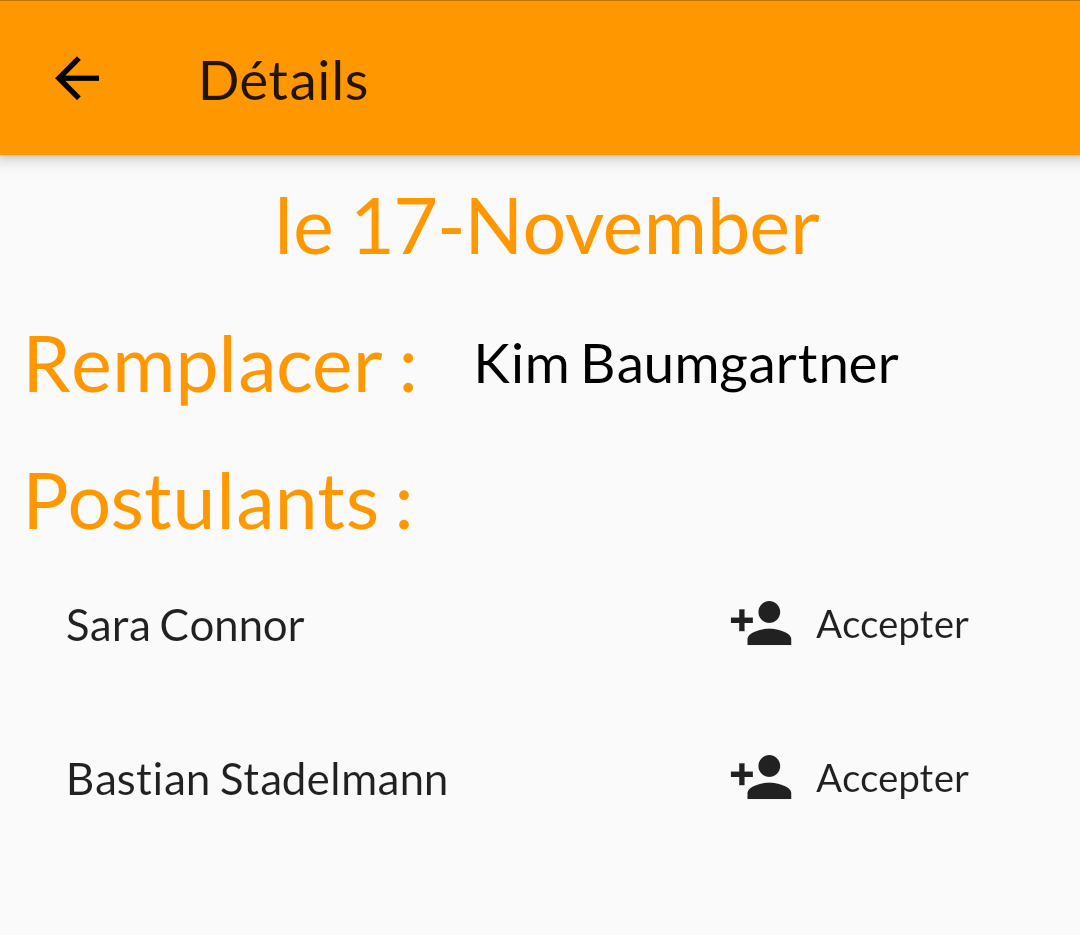
\includegraphics[width=0.6\linewidth]{screenshots/scenario_03/detail_auth.png}
            \caption{ayant mis le service en bourse}
            \label{fig:detail_auth}
        \end{subfigure}
        \begin{subfigure}{.45\textwidth}
            \centering
            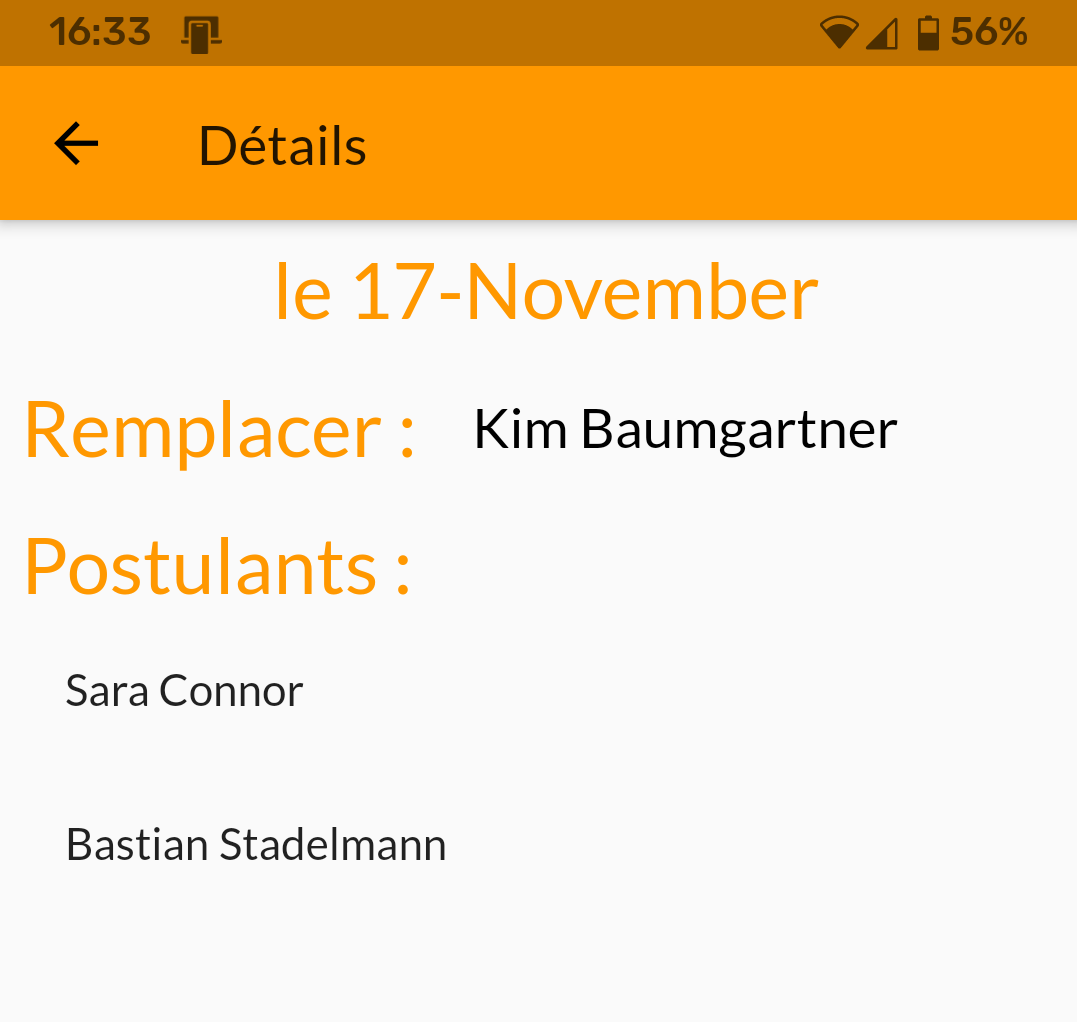
\includegraphics[width=0.6\linewidth]{screenshots/scenario_03/detail_non_auth.png}
            \caption{autre}
            \label{fig:detail_non_auth}
        \end{subfigure}
        \caption{scénario III}
        \label{fig:scen03}
    \end{figure}

    S'il s'agit de l'utilisateur ayant mis le service en bourse à l'occurence Kim, l'écran détails tel que \ref{fig:detail_auth} s'affiche.
    S'il s'agit de n'importe quel autre utilisateur alors l'écran détails s'affiche comme dans \ref{fig:detail_non_auth}

    Ainsi, seul l'utilisateur ayant mis le service en bourse est en mesure d'accpter un ou une remplaçante. Pour se faire,
    Kim doit appuyer sur le bouton accepter de la personne de son choix.

\section[Valider un échange - Scénario IV]{Scénario IV}
    \subsection*{Valider un échange}
    Toujours dans la continuation de notre exemple, nous allons voir ici 
    la validation d'un échange. En effet, même si un utilisateur
    à accepté un remplaçant pour son service. Il faut encore que cette
    transaction soit validée par un utilisateur avec privilèges.

    Il existe trois types d'utilisateurs:
    \begin{center}
        \begin{tikzpicture}
            \node[] at (0.5,2) {normal};
            \draw[color=RoyalRed] (2,2) circle (3.5cm);
            \node[] at (2.5,1.5) {manager};
            \draw[color=RoyalRed] (1,2) circle (2.5cm);
            \node[] at (4.5,1.0) {admin};
            \draw[color=RoyalRed] (0,2) circle (1.5cm);
        \end{tikzpicture}
    \end{center}
    
